Throughout this chapter, core terms and concepts that are essential to the understanding of this thesis are explained. First, networks-on-chip are
described, as this whole work builds upon and analyzes them. Afterwards, fundamental concepts of information security and their relevance for this
thesis are outlined. Finally, essential aspects of the communication strategy devised in this thesis are delineated.

\section{Networks-On-Chip}\label{sec:networkonchipfun}
\textit{Networks-on-Chip \glspl{noc})} are a paradigm for interconnecting components on a chip. They are employed on
\textit{Multi-Processor Systems-on-Chip (\glspl{mpsoc})} \cites(e.g.)(){ivanov05nocintroduction}{biswas15routerattack}{tatas16designingnocs}, where they
provide the communication infrastructure for the \textit{processing elements} and other \textit{intellectual property (\gls{ip}) cores}\footnote{The
term \textit{\gls{ip} cores} encompasses many kinds of chip components. Besides processing elements, it includes e.g. memory nodes and
hardware accelerators.}. The basic concept is to incorporate many point-to-point connections between neighboring cores, breaking with the traditional
concept of global interconnection buses. After describing the internal structure of \glspl{noc} in the following paragraphs, the advantages of this
approach will be explained.

In recent research, the topology of a \gls{noc} is usually assumed to be a 2D mesh
\cites(e.g.)(){frey17hardenednoc}{kumar02networkonchip}{fernandes16nocrouting}{boraten16packetsecurity}. While this is not a
requirement\footnote{Other \gls{noc} topologies include e.g. 2D folded tori and 3D meshes \cite[2]{feero07noc3d}.}, it is both convenient
to work with and applicable in practice. Thus, in this thesis, the network nodes are also laid out in this manner.
In a 2D mesh, each node is connected to its four neighbors (excluding the ones located at the boundaries).

A node consists of a processing element\footnote{As already mentioned, other types of cores are also possible. Since only processing elements are of
relevance to this thesis, no further distinctions will be made.}, a network interface, and a router \cite{dally01routepacketsnotwires}. The processing
element executes applications, requiring it to be able to send and receive messages. The network interface facilitates this by connecting the
processing element to the router. Finally, the router manages the connections to neighboring nodes and the local processing element. An example of
this architecture is given in Figure \vref{fig:nocexample}.

\begin{figure}
    \centering
    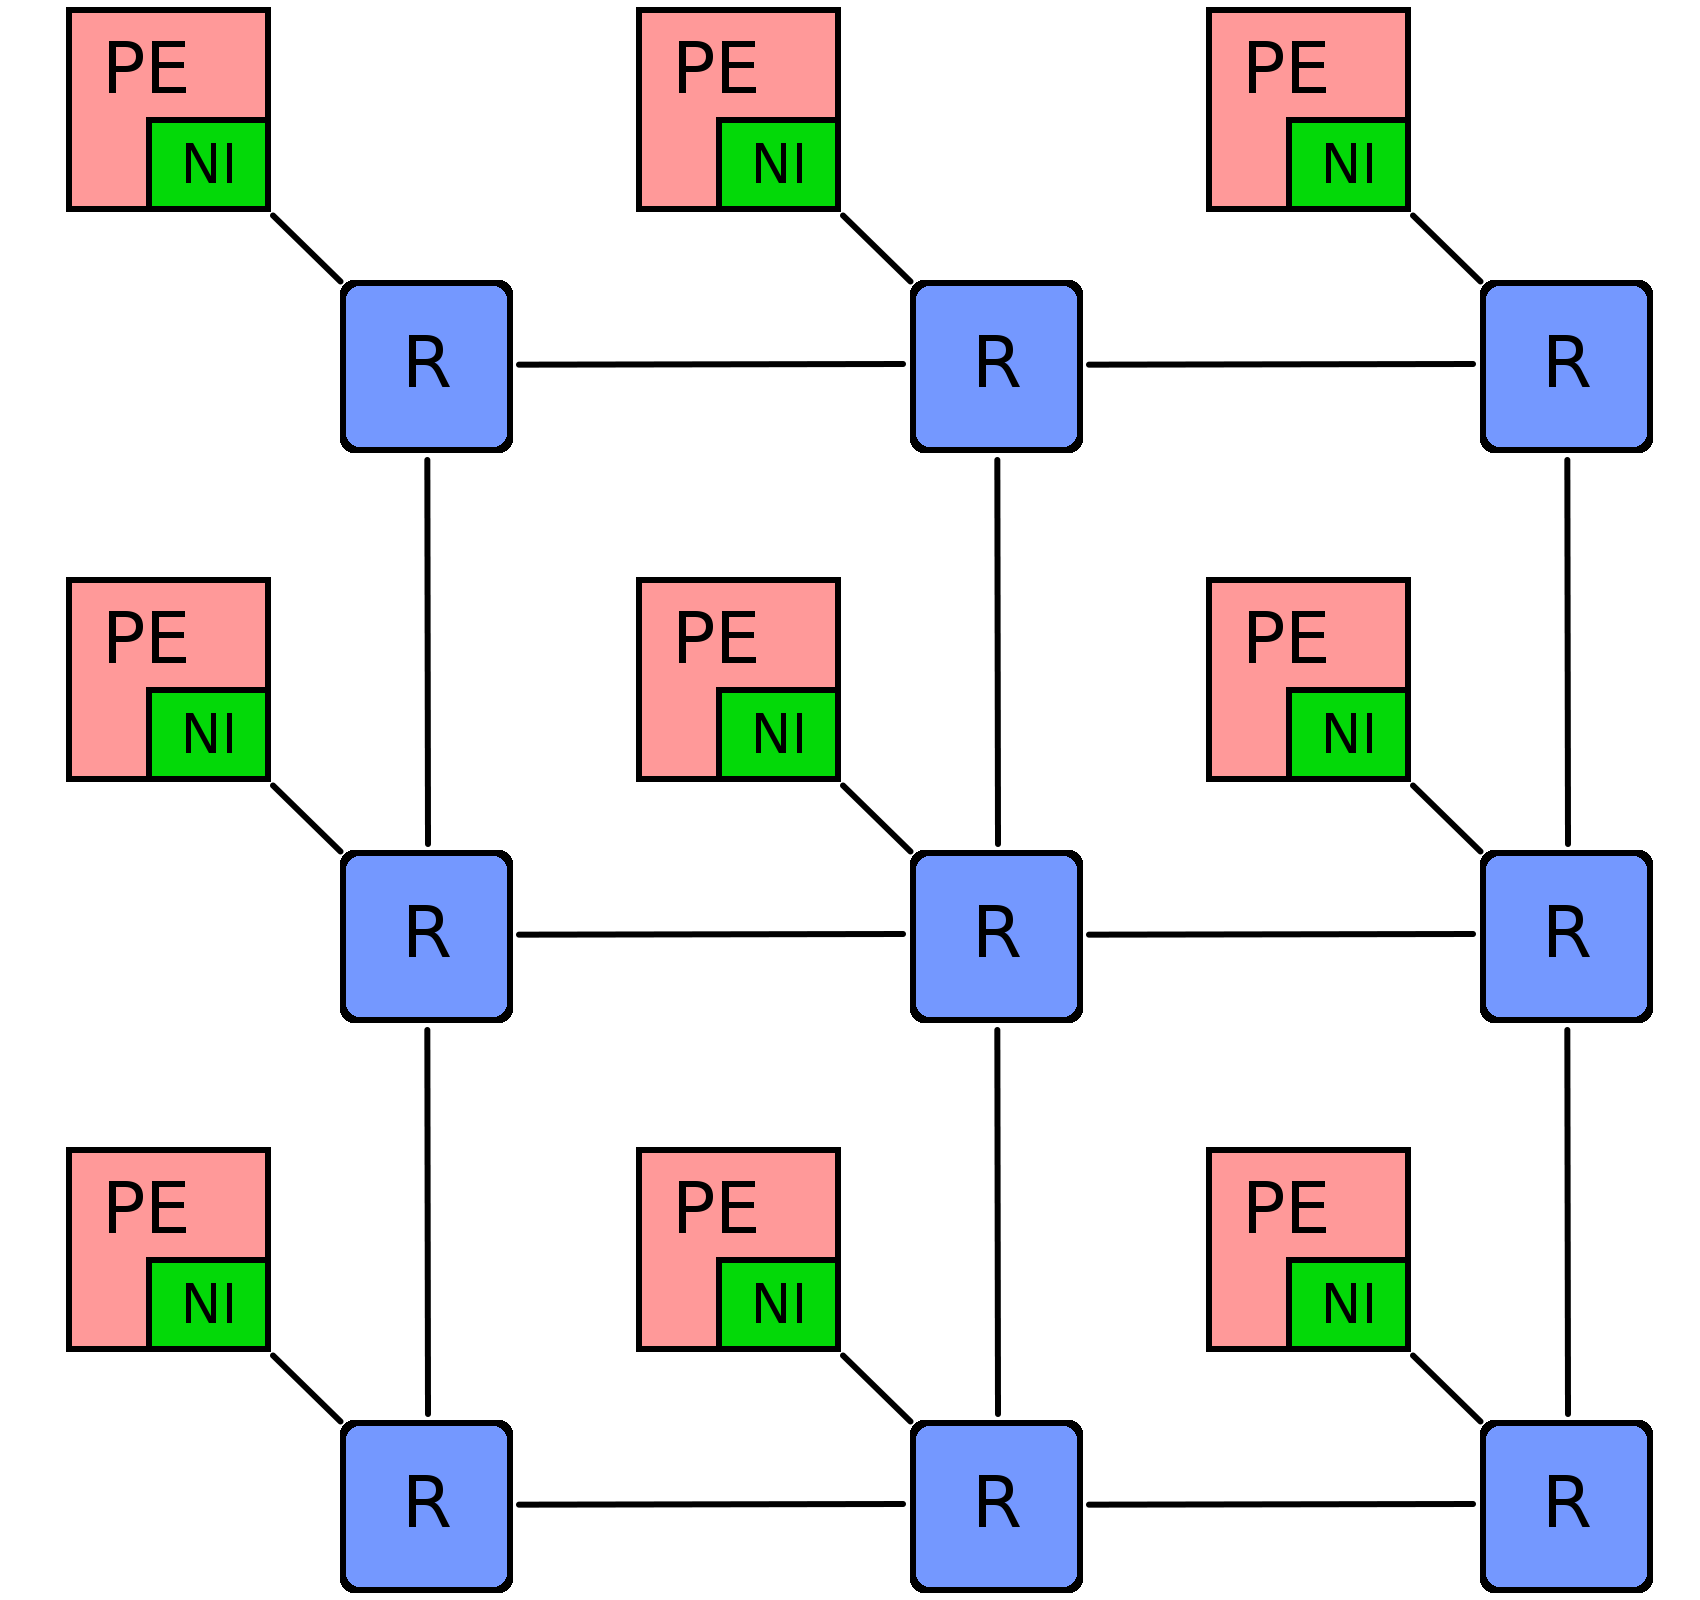
\includegraphics[width=0.6\textwidth]{noc-3x3-colored}
    \caption[Example of a 3x3 mesh NoC]{Example of a Network-on-Chip in a 2D mesh topology of size 3x3. The processing elements (red) contain a network interface
    (green) through which they are connected to a router (blue). The routers are interconnected as a 2D mesh.}
    \label{fig:nocexample}
\end{figure}

Compared to traditional bus-based interconnect systems, \glspl{noc} provide a lot of advantages\footnote{There are disadvantages entailed by
the use of \glspl{noc} over bus-based systems, but research has shown them to be outweighed by the benefits. \citeauthor{tatas16designingnocs}
\cite{tatas16designingnocs} give a detailed comparison.}, especially for many-core systems
\cite[5\psqq]{tatas16designingnocs}. A significant advantage is scalability: since the cores do not share a global bus, \enquote{local performance is not
degraded} \cite[6]{tatas16designingnocs} as more components are added, and \enquote{aggregated bandwidth scales with the network size}
\cite[6]{tatas16designingnocs}.

In addition, the absence of global interconnection wires facilitates the use of different clock domains. This enables the implementation of the
\textit{globally asynchronous, locally synchronous (\gls{gals})} paradigm, which becomes increasingly important in chip design due to the growing
number of cores and resulting timing closure issues \cites[3]{kumar02networkonchip}[2]{ivanov05nocintroduction}.

Furthermore, the constantly increasing design complexity of modern chips \cite{mack11mooreslaw} renders specialized on-chip
interconnections infeasible to implement. Designing such a system \enquote{would take too much time and mapping of applications to dedicated
architectures would be impossible} \cite[1]{kumar02networkonchip}. In contrast, \glspl{noc} are intended to be general purpose interconnect systems; they
\enquote{facilitate […] modularity by defining a standard interface} \cite[1]{dally01routepacketsnotwires}.

When utilizing \gls{noc} architectures in practice, it is crucial that they allow for an efficient implementation and swift communications. The
former is attained by reducing the chip area requirements and power consumption as much as possible, while the latter is realized
through low electronic delays and message transmission latencies. To achieve this, all components of the \gls{noc} need to be optimized regarding
these criteria. In this thesis, several approaches like specifically lightweight cryptographic algorithms and single-cycle routing are pursued to
meet them. They are explained in detail in Sections (insert refs here).% TODO: refs to relevant sections with details

\section{Protection Goals}\label{sec:protectiongoals}
% Confidentiality, integrity, availability
Protection goals describe desired properties of a system with regard to information security. They are divided into \textit{confidentiality},
\textit{integrity}, and \textit{availability}\footnote{The goals may be further classified to include e.g. \textit{unobservability} or \textit{plausible
deniability}. However, these are extraneous to this thesis.}. Confidentiality is achieved by preventing unauthorized access to information, which
can be accomplished e.g. by means of encryption. Integrity is attained by ensuring that any unintentional modifications to information, both accidental and
malicious, are detected, e.g. through authentication techniques. Finally, availability refers to the reliable accessibility of information. It is
achieved via methods like backup systems and redundant hardware.

In \gls{noc} architectures, it is naturally desirable to fulfill these goals\footnote{The necessity for security measures was demonstrated in
related research, which is elaborated in Section \ref{sec:nocsecurity}.}. In this thesis, confidentiality and integrity through encryption and
authentication are examined.

\section{Hardware Trojans}\label{sec:hardwaretrojans}
% What are HTs, why can they get into other hardware, what are their properties
% TODO: third party IP nicht der einzige Grund
Hardware trojans are \enquote{malicious modifications of electronic hardware} \cite[1]{bhunia14hardwaretrojans} intended to disrupt normal
system behavior or to extract sensitive information. The introduction of hardware trojans into larger systems (such as \glspl{mpsoc}) is possible
through a number of different infection vectors (see Section \ref{sec:necessityofsecurity} for details).

In order to remain undetected, attackers aim to construct hardware trojans that are \enquote{stealthy in nature} \cite[1]{bhunia14hardwaretrojans}
and \enquote{evade […] detection through conventional postmanufacturing test} \cite[1]{bhunia14hardwaretrojans}. Hardware trojans are usually in a
dormant state until they are activated by a trigger signal to carry out their task \cites{bhunia14hardwaretrojans}{ancajas14fortnocs}. While the
trojan is inactive, communications through the \gls{noc} are unaffected and the system operates normally.

Attack types: information leak/eavesdropping, DoS (→ bandwidth depletion, deadlock, livelock)
% TODO: is this a fundamental? or write this when describing our attacker model?

\section{Flits}\label{sec:flits}
\textit{Flow control units (flits)} are small pieces of data that are sent over a network. They are usually created by breaking a larger
packet down into parts to allow for their individual transmission \cite[6]{flitslecturecmu}. Each flit must contain a set of header fields (such as source and
destination address, sequence number, or identifier) that are required for routing and handling by the receiver \cite[2]{flitslectureutah}.
In addition, it contains a payload that carries the actual information to be transmitted.

In the context of \glspl{noc}, flits are often used as the standard unit of transmission \cite[51\psqq]{tatas16designingnocs}. Details on how flits
are used in this thesis can be found in (insert section/chapter vref).
% TODO: insert reference
% TODO: "used in this thesis" correct?

\section{Automatic Repeat Requests}\label{sec:arqs}
When reliable data transmissions over an unreliable network are desired, the communication protocol needs to ensure that all packets arrive unmodified
at their intended destinations. A common way to achieve this is the usage of \textit{automatic repeat requests (\glspl{arq})}.

In traditional implementations, such as \gls{tcp}, the receiver confirms the arrival of packets by answering each one with an acknowledgment.
If the sender does not receive a confirmation within a given time span, the corresponding packet is assumed lost and automatically retransmitted.

A \gls{noc} is considered an unreliable network in this thesis. One reason for this is potential network congestion, which can lead to high latencies
and dropped flits. Another possibility is compromised, malicious routers that drop or modify flits to disrupt the normal network operations, e.g. as part of a
\gls{dos} attack.

In this thesis, there are no acknowledgments for successfully transmitted flits. Instead, the receiver informs the sender of missing or corrupted
flits by issuing an \gls{arq} back to the sender. Upon arrival, the sender will retransmit the flits in question. In combination with
authentication techniques, this aids in fulfilling the protection goal of integrity. This scheme is described in detail in Section
\ref{sec:retransmissions}.

\section{Network Coding}\label{sec:networkcodingfun}
Network coding is a technique for transmitting packets efficiently over a network. First described in 2000 by \citeauthor{ahlswede00networkflow}
\cite{ahlswede00networkflow}, the idea is to maximize the information flow through a network and achieve higher throughput than traditional transmission
schemes. It is achieved by allowing intermediate network nodes to encode incoming packets before passing them on, creating combinations of different
packets in the process. At the destinations, the received data can be decoded again to obtain the original packets. Traditionally, network coding is
used in multicast communication patterns, but it has also been applied successfully to unicast scenarios \cite[e.g.][]{moriam15manycorenc}.

A popular coding scheme, dubbed \textit{linear network coding} \cite{li03linearnc}, is to regard all packets arriving at a node from different incoming links as a vector.
Then, linear transformations can be applied to it to obtain new combinations to send out \cite[1]{li03linearnc}. To allow receivers to decode the
combinations into the original packets, the encoding patterns applied at each node can be \enquote{agreed upon beforehand} \cite[1]{li03linearnc}.
However, this requires global knowledge of the network topology. A practical alternative is to attach the encoding information to the packets in the
form of a \textit{global encoding vector (\gls{gev})} \cites[2\psqq]{chou03practicalnc}[5\psq]{chou07ncforinternetandwireless} that is updated at each intermediate node to
represent the current encoding pattern.

In addition to increasing the network performance by maximizing throughput, network coding can also provide an additional layer of resilience against
malicious intermediate nodes. It facilitates \enquote{a natural way to take advantage of multipath diversity for security against wiretapping attacks}
\cite[8]{fragouli07ncfundamentals} and can also be helpful against active attackers.

During this thesis, network coding is used primarily as a means of resilience against attackers. Furthermore, only the sender nodes will compute
combinations of different flits, while intermediate nodes merely forward them. Section (insert vref here) illuminates this subject in detail.
% TODO: mention that mostly used with multicast, we do unicast
% TODO: mention PNC paper, that we use RLNC, but only senders encode and create generations ("only intra-session network coding")
% TODO: insert vref
